\begin{center}
	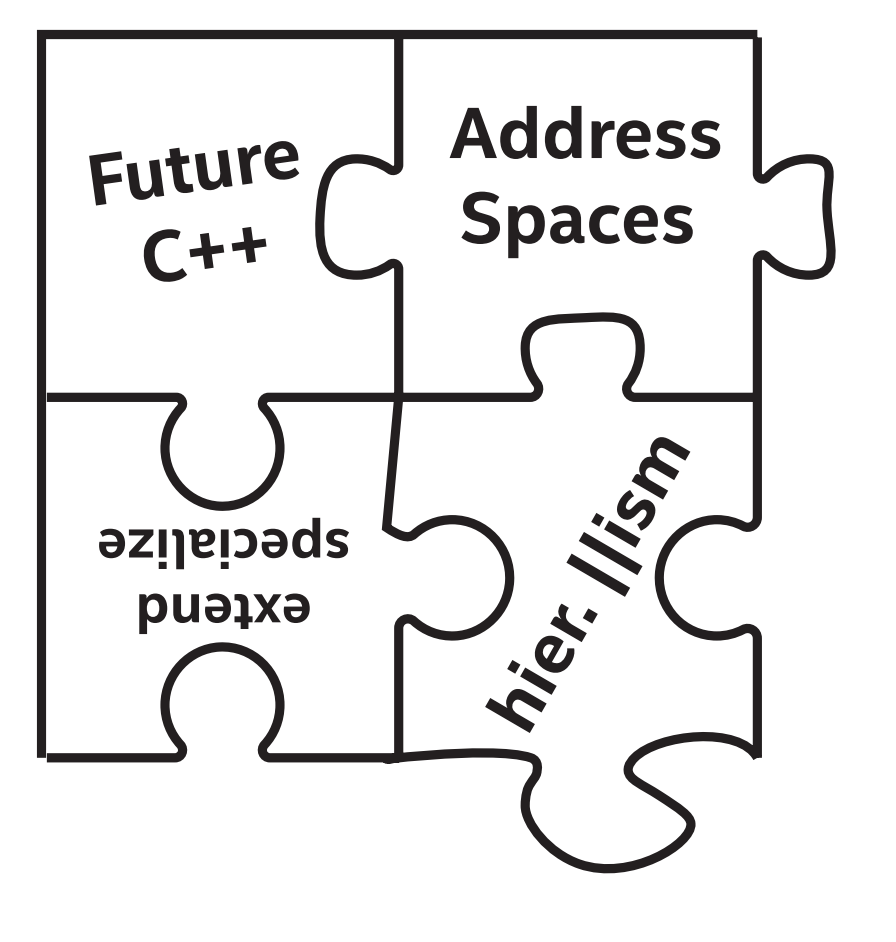
\includegraphics[width=0.5\textwidth]{content/chapter-20/images/1}
\end{center}

Take a moment now to feel the peace and calm of knowing that we finally understand everything about programming using SYCL and DPC++. All the puzzle pieces have fallen into place.\par

Before we get too comfortable, let’s note that this book was written at an exciting time for SYCL and DPC++. It has been a period of rapid development that coincided with the release of the first DPC++ specification and the SYCL 2020 provisional specification. We’ve endeavored to ensure that the code samples, in all previous chapters, compile with the open source DPC++ compiler at the time that this book was sent to publication (Q3 2020) and execute on a wide range of hardware. However, the future-looking code shown in this epilogue does not compile with any compiler as of mid-2020.\par

In this epilogue, we speculate on the future. Our crystal ball can be a bit difficult to read—this epilogue comes without any warranty.\par

The vast majority of what this book covers and teaches will endure for a long time. That said, it is too hot of an area for it to remain at rest, and changes are occurring that may disrupt some of the details we have covered. This includes several items that appeared first as vendor extensions and have since been welcomed into the specification (such as sub-groups and USM). That so many new features are on track to become part of the next SYCL standard is fantastic, but it has made talking about them complicated: should we refer to such features as vendor extensions, experimental/provisional features of SYCL, or part of SYCL?\par

This epilogue provides a sneak peek of upcoming DPC++ features that we are very excited about, which were unfortunately not quite finished at the time we sent the book to be published. We offer no guarantees that the code samples printed in this epilogue compile: some may already be compatible with a SYCL or DPC++ compiler released after the book, while others may compile only after some massaging of syntax. Some features may be released as extensions or incorporated into future standards, while others may remain experimental features indefinitely. The code samples in the GitHub repository associated with this book may be updated to use new syntax as it evolves. Likewise, we will have an erratum for the book, which may get additions made from time to time. We recommend checking for updates in these two places (code repository and book errata—links can be found early in Chapter 1).\par
